%% bpmlr.tex
%% V0.1
%% 2015/01/01
%% by Mack Sweeney

\documentclass[10pt]{proc}


% *** CITATION PACKAGES ***
%
\usepackage{cite}

% *** OTHER BIBLIOGRAPHY PACKAGES ***
%
%\usepackage[numbers]{natbib}


% *** GRAPHICS RELATED PACKAGES ***
%
\usepackage[pdftex]{graphicx}
% declare the path(s) where your graphic files are
\graphicspath{{./graphics/}}
% and their extensions so you won't have to specify these with
% every instance of \includegraphics
\DeclareGraphicsExtensions{.pdf,.jpeg,.png}

\usepackage{scalerel}
\usepackage{mdframed}

% For graphical models:
\usepackage{tikz}
\usetikzlibrary{bayesnet}


% *** MATH PACKAGES ***
%
\usepackage[cmex10, fleqn]{amsmath}
\usepackage{bm}
\usepackage{bbm}
\usepackage{amssymb}
\usepackage{mathtools}
\usepackage{etoolbox}
%
% Also, note that the amsmath package sets \interdisplaylinepenalty to 10000
% thus preventing page breaks from occurring within multiline equations. Use:
\interdisplaylinepenalty=2500
% after loading amsmath to restore such page breaks as IEEEtran.cls normally
% does. amsmath.sty is already installed on most LaTeX systems.


% *** SPECIALIZED LIST PACKAGES ***
%
\usepackage{algorithm}
\usepackage[noend]{algpseudocode}


% *** ALIGNMENT PACKAGES ***
%
\usepackage{array}
\usepackage{booktabs}


% *** SUBFIGURE PACKAGES ***
%\usepackage[tight,footnotesize]{subfigure}
%\usepackage[caption=false]{caption}
%\usepackage[font=footnotesize]{subfig}
\usepackage[caption=false,font=footnotesize]{subfig}


% *** FLOAT PACKAGES ***
%
\usepackage{fixltx2e}
\usepackage{stfloats}


% *** PDF, URL AND HYPERLINK PACKAGES ***
%
\usepackage{url}


% BEGIN PAPER CONTENT
%
\title{Nonparametric Biased Mixtures of Linear Regressions}
\author{
    Mack Sweeney, Carlotta Domeniconi, Kathryn Laskey, Huzefa Rangwala\\
        George Mason University
}
\date{\today}


% New commands to be used in this report.
\newcommand*{\Scale}[2][4]{\scalebox{#1}{$#2$}}%
\newcommand*{\Resize}[2]{\resizebox{#1}{!}{$#2$}}%
\newcommand{\norm}[1]{\left\lVert#1\right\rVert}
\newcommand{\pluseq}{\mathrel{+}=}
\newcommand{\mineq}{\mathrel{-}=}
\newcommand{\asteq}{\mathrel{*}=}
\newcommand{\elips}[1]{\ldots#1\allowbreak}
\newcommand{\bc}{,\allowbreak}

\AtBeginEnvironment{align}{\par\footnotesize}
\AfterEndEnvironment{align}{\normalsize}
\AtBeginEnvironment{align*}{\par\footnotesize}
\AfterEndEnvironment{align*}{\normalsize}

\newtheorem{lemma}{Lemma}
\newtheorem{proof}{Proof}


\begin{document}
\maketitle


\begin{abstract}

\end{abstract}


\section{Introduction}

Navigating a university degree program is a duanting task. There are often
several categories of requirements that need to be met, each with several
courses to choose from. Students wish to choose courses that will meet these
requirements. They also want to avoid taking courses so difficult they are
unable to learn the material and perform well.

This selection task is complicated by the fact that students take multiple
courses each semester. Taking one particularly difficult course may be an
exciting challenge, while taking two or three concurrently would be
overwhelming. So there is a need to properly blend courses of varying difficulty
in a single semester. Certain course combinations may also be very
complementary. Many courses are associated with labs, which provide practical
experience with the theoretical lecture concepts.

This task is also complicated by the sequential nature of learning. Many courses
build upon knowledge learned in previous courses. Some courses can only be taken
if the student has already taken the prerequisite courses. Other courses do not
have these requirements but should still not be taken unless certain
prerequisite knowledge has been learned. If no prerequisites are given, students
must determine for themselves which prior courses should have been taken in
order to do well in a course currently being selected.

Beyond the questions of difficulty and requirements, students would also like to
explore their individual interests as much as possible. With all else being
equal between two courses, the student will choose the most interesting one.
Sometimes personal interest will also lead students to take a course which is
more difficult but meets the same requirement as an easier course. This
subjective factor makes it impossible for a one-size-fits-all course selection
to be successful.

We seek to address one particular aspect of the degree planning problem.
We seek to assist students in ranking courses for a particular semester given
all prior course data for all students in the university. In this study, we rank
these courses based on student-relative difficulty

\section{Problem Formulation}\label{problem-formulation}

In the traditional university setting, cohorts of students are admitted and
begin taking courses. Each semester, students can enroll in zero or more courses
and earn grades in each course. These grades are assigned on a 0-100 scale. At
the end of the course, the final grades are binned into categorical values on
the A-F scale (A, A-, B+, B, ..., C, C-, D, F). These categorical values are
often mapped to a numerical categorical scale of 4-0 for grade point average
(GPA) calculations.

Our dataset consists of polyadic relationships resulting from students taking
courses over a sequence of semesters. Each record is uniquely identified by the
student id (sid), course id (cid), and a chronological semester number (term).
We can organize these triads into a sparse tensor $\bm{Y} \in \mathbb{R}^{N
\times M \times T}$. $N$ is the number of unique students in the dataset,
$M$ the number of unique courses, and $T$ the number of terms. So entry
$\bm{Y}_{n,m,t} \in [0, 4]$ represents the grade student $n$ earned in course
$m$ during semester $t$. These grades are ordinal values in the range 0 to 4.

We also observe various pieces of \textit{side information} for each observed triad.
Side information includes observations aside from the grade that describe the
entities of the triad (student, course, term) or their interaction.  For
instance, student side information includes demographics. Course side info
includes attributes of the instructor. Term side info might include
university-wide statistics from that term or previous terms. Side info
describing interactions is rich and diverse. Two examples are the number of
credit hours a student is enrolled in during the term and a student's past
performance in all courses of the same discipline. We extract $f$ features from
the side info and assemble it into a sparse tensor $\bm{X} \in \mathbb{R}^{n
\times m \times t \times f}$.

We often want to split our database into train and test sets. We assume
the train set is unobserved and make predictions about the unobserved test set.
For this purpose, we define $Y^{(t)}$ to be the cumulative grade matrix up to
and including term $t$. We define this recursively:
%
\begin{enumerate}
    \item  $Y^{(0)} = \bm{Y}_{*,*,0}$
    \item  $Y^{(t)} = join(Y^{(t-1)}, \bm{Y}_{*,*,t})$,
\end{enumerate}
%
where $join$ is an inner-join on the (cid, sid, term) fields. Conflicts are
resolved by keeping the values from the more recent term. We define
$\bm{X}^{(t)}$ to be the cumulative feature vector matrix, recursively
accumulated in the same manner.

Given the cumulative grade matrix $Y^{(t-1)}$ and feature vector
matrix $\bm{X}^{(t-1)}$, our task is to predict the unobserved grades in term
$t$.

\section{Modeling}\label{model}

We build a model that (1) accurately predicts next-term grades given data from
previous terms, (2) clusters students to identify common learner profiles, and
(3) is highly interpretable. We derive a fully Bayesian probabilistic model that
combines mixtures of linear regressions with nonparametric model selection.
Throughout this section, we assume we are currently in term $t$ and have been
given data for terms up to $t-1$. We leave off the term superscript, so $Y$
represents $Y^{(t-1)}$ and $\bm{X}$ represents $X^{(t-1)}$.

We model the actual real-valued 0-100 grades as latent variables $G_{nm}$. The
observed grades $Y_{nm}$ are obtained by thresholding $G_{nm}$ using fixed
cutoffs $\bm{\gamma}$:
%
\begin{align}
    Y_{nm} &= l \text{ iff } \bm{\gamma}_l \ge G_{nm} < \bm{\gamma}_{l+1}, \\
         l &\in \{\text{F, D, C-, C, C+, B-, B, B+, A-, A} \}.
\end{align}
%
The actual choice of cutoffs $\bm{\gamma}$ is unimportant; the model will adjust
the distribution of $G_{nm}$ across the thresholded space appropriately during
learning. We choose a cutoff scheme common in undergraduate curriculums:
%
\begin{align}
    \bm{\gamma} = \{ 60, 70, 73, 77, 80, 83, 87, 90, 93, 100, \infty \}.
\end{align}

We assume there are latent clusters of students, such that each student belongs
to one cluster. We model these latent memberships with indicator variables
$Z_n = k$ drawn from a multinomial with parameter $\pi$. We place a Dirichlet
distribution on $\pi$ with parameter $\alpha$. The distribution of grades within
a cluster is modeled using a Gaussian linear regression. So for each cluster, we
have regression coefficients $\beta_k$ and covariance matrix $\Sigma_k$.
Students have varying levels of competency and courses have varying difficulty.
So we offset the regression by student- and course-specific univariate Gaussian
bias terms $s_n$ and $c_m$. We place a conjugate Guassian Inverse-Wishart (GIW)
prior on $\beta_k$ and $\Sigma_k$.
%
\begin{align}
    \pi &\sim \text{Dirichlet}\left(
        \frac{\alpha}{K}, ..., \frac{\alpha}{K}
    \right)  \\
    Z_n | \pi &\sim \text{Mult}\left(
        \pi_1, ..., \pi_k
    \right)  \\
    \Sigma_k &\sim IW\left(
        \nu_0, S_0
    \right)  \\
    \beta_k &\sim \mathcal{N}\left(
        \beta_0, \frac{1}{\kappa_0} \Sigma_k
    \right)  \\
    s_n &\sim \mathcal{N}\left(
        \mu_s, \sigma_s^2
    \right)  \\
    c_m &\sim \mathcal{N}\left(
        \mu_c, \sigma_c^2
    \right)  \\
    G_{nm} | Z_n, X_{mn} &\sim \mathcal{N}\left(
        \beta_k X_{nm}^T + s_n + c_m, \Sigma_k
    \right)
\end{align}


% Finite model
\begin{figure}[th!]
  \centering
  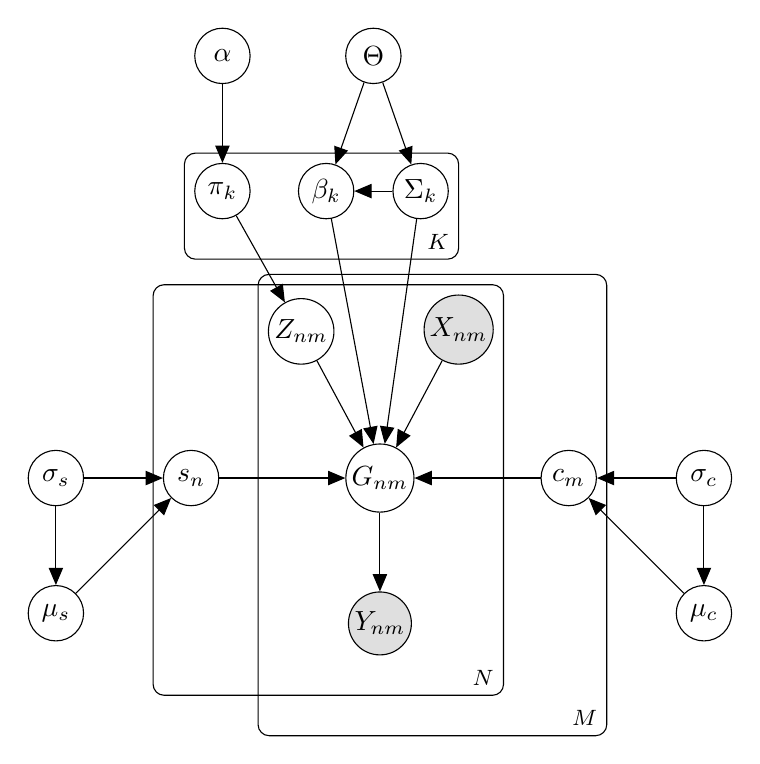
\begin{tikzpicture}

    % Define nodes
    \node[obs]                                (Y) {$Y_{nm}$};
    \node[latent, above=of Y]                 (G) {$G_{nm}$};
    \node[latent, above=of G, xshift=-1cm]    (Z) {$Z_{nm}$};
    \node[obs, above=of G, xshift=1cm]        (X) {$X_{nm}$};

    \node[latent, left=of G, xshift=-0.6cm]   (s) {$s_n$};
    \node[latent, left=of s]                  (ss) {$\sigma_s$};
    \node[latent, below=of ss]                (ms) {$\mu_s$};

    \node[latent, right=of G, xshift=0.6cm]   (c) {$c_m$};
    \node[latent, right=of c]                 (sc) {$\sigma_c$};
    \node[latent, below=of sc]                (mc) {$\mu_c$};

    \node[latent, above=of Z, xshift=-1cm]    (pi) {$\pi_k$};
    \node[latent, above=of pi]             (alpha) {$\alpha$};
    \node[latent, right=of alpha, xshift=0.2cm]  (theta) {$\Theta$};

    \node[latent, below=of theta, xshift=-0.6cm] (beta) {$\beta_k$};
    \node[latent, below=of theta, xshift=0.6cm]  (sk) {$\Sigma_k$};

    % Connect the nodes
    \edge {G} {Y};
    \edge {s,c,Z,X,beta,sk} {G};
    \edge {ss,ms} {s};
    \edge {ss} {ms};
    \edge {sc,mc} {c};
    \edge {sc} {mc};

    \edge {pi} {Z};
    \edge {sk} {beta};
    \edge {alpha} {pi};
    \edge {theta} {beta,sk};

    % Plates
    \plate {student} {(s)(Z)(X)(G)(Y)} {$N$};
    \plate {course} {(c)(Z)(X)(G)(Y)(student.south east)(student.north east)} {$M$};
    \plate {comps} {(pi)(beta)(sk)} {$K$};

  \end{tikzpicture}
  \vspace{2pt}
  \caption{Finite Bayesian Mixture of Linear Regressions. The hyper-parameters
           $\Theta = (\beta_0, \kappa_0, \nu_0, \Sigma_0)$}
  \label{fig:finite-bpmlr}
\end{figure}

This model shares the problem of all finite mixture models: how do we select the
optimal number of mixture components $K$? We can bypass this problem by
replacing our Dirichlet prior with a Dirichlet process (DP) prior. The Dirichlet
process is a distribution over distributions, allowing us to represent a
countably infinite mixture of linear regressions. The DP has concentration
parameter $\alpha$ and base distribution $H_0$. So we replace (4-7) above with:
%
\begin{align}
    \pi | H &\sim H  \\
    H | H_0, \alpha &\sim DP(H_0, \alpha)  \\
    H_0 | \Theta &\sim \mathcal{N}\left(
        \beta_0, \frac{1}{\kappa_0} \Sigma_k
    \right) \times IW(\nu_0, \Sigma_0) \\
    \beta_k, \Sigma_k &\sim H_0
\end{align}


% Infinite model.
\begin{figure}[th!]
  \centering
  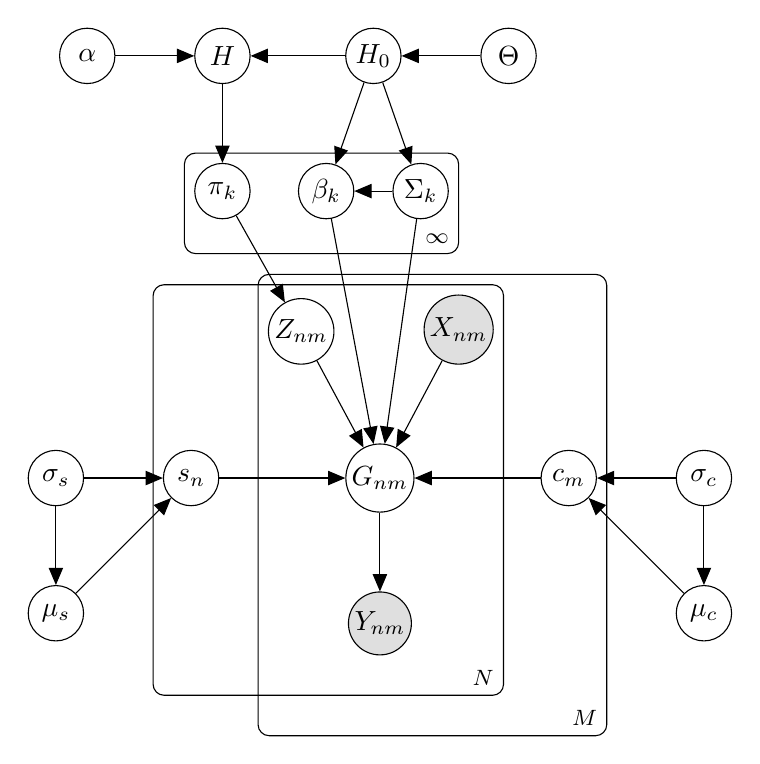
\begin{tikzpicture}

    % Define nodes
    \node[obs]                                (Y) {$Y_{nm}$};
    \node[latent, above=of Y]                 (G) {$G_{nm}$};
    \node[latent, above=of G, xshift=-1cm]    (Z) {$Z_{nm}$};
    \node[obs, above=of G, xshift=1cm]        (X) {$X_{nm}$};

    \node[latent, left=of G, xshift=-0.6cm]   (s) {$s_n$};
    \node[latent, left=of s]                  (ss) {$\sigma_s$};
    \node[latent, below=of ss]                (ms) {$\mu_s$};

    \node[latent, right=of G, xshift=0.6cm]   (c) {$c_m$};
    \node[latent, right=of c]                 (sc) {$\sigma_c$};
    \node[latent, below=of sc]                (mc) {$\mu_c$};

    \node[latent, above=of Z, xshift=-1cm]    (pi) {$\pi_k$};

    \node[latent, above=of pi]                (H) {$H$};
    \node[latent, left=of H]                  (alpha) {$\alpha$};
    \node[latent, right=of H, xshift=0.2cm]   (H0) {$H_0$};
    \node[latent, right=of H0]                (theta) {$\Theta$};

    \node[latent, below=of H0, xshift=-0.6cm] (beta) {$\beta_k$};
    \node[latent, below=of H0, xshift=0.6cm]  (sk) {$\Sigma_k$};

    % Connect the nodes
    \edge {G} {Y};
    \edge {s,c,Z,X,beta,sk} {G};
    \edge {ss,ms} {s};
    \edge {ss} {ms};
    \edge {sc,mc} {c};
    \edge {sc} {mc};

    \edge {pi} {Z};
    \edge {sk} {beta};
    \edge {H} {pi};
    \edge {alpha} {H};
    \edge {H0} {H,beta,sk};
    \edge {theta} {H0};

    % Plates
    \plate {student} {(s)(Z)(X)(G)(Y)} {$N$};
    \plate {course} {(c)(Z)(X)(G)(Y)(student.south east)(student.north east)} {$M$};
    \plate {comps} {(pi)(beta)(sk)} {$\infty$};

  \end{tikzpicture}
  \vspace{2pt}
  \caption{Infinite Bayesian Mixture of Linear Regressions. The hyper-parameters
           $\Theta = (\beta_0, \kappa_0, \nu_0, \Sigma_0)$}
  \label{fig:infinite-bpmlr}
\end{figure}



\section{Experiments}\label{experiments}

\section{Analysis}\label{analysis}

\section{Previous work}\label{previous work}

\section{Conclusions}\label{conclusions}
We worked hard, and achieved very little.

% use section* for acknowledgement
\section*{Acknowledgment}
This research was funded by NSF IIS grant 1447489.


\bibliographystyle{siam}
\bibliography{refs}

\end{document}

